% Options for packages loaded elsewhere
% Options for packages loaded elsewhere
\PassOptionsToPackage{unicode}{hyperref}
\PassOptionsToPackage{hyphens}{url}
\PassOptionsToPackage{dvipsnames,svgnames,x11names}{xcolor}
%
\documentclass[
  british,
  a4paper,
]{article}
\usepackage{xcolor}
\usepackage{amsmath,amssymb}
\setcounter{secnumdepth}{-\maxdimen} % remove section numbering
\usepackage{iftex}
\ifPDFTeX
  \usepackage[T1]{fontenc}
  \usepackage[utf8]{inputenc}
  \usepackage{textcomp} % provide euro and other symbols
\else % if luatex or xetex
  \usepackage{unicode-math} % this also loads fontspec
  \defaultfontfeatures{Scale=MatchLowercase}
  \defaultfontfeatures[\rmfamily]{Ligatures=TeX,Scale=1}
\fi
\usepackage{lmodern}
\ifPDFTeX\else
  % xetex/luatex font selection
\fi
% Use upquote if available, for straight quotes in verbatim environments
\IfFileExists{upquote.sty}{\usepackage{upquote}}{}
\IfFileExists{microtype.sty}{% use microtype if available
  \usepackage[]{microtype}
  \UseMicrotypeSet[protrusion]{basicmath} % disable protrusion for tt fonts
}{}
\makeatletter
\@ifundefined{KOMAClassName}{% if non-KOMA class
  \IfFileExists{parskip.sty}{%
    \usepackage{parskip}
  }{% else
    \setlength{\parindent}{0pt}
    \setlength{\parskip}{6pt plus 2pt minus 1pt}}
}{% if KOMA class
  \KOMAoptions{parskip=half}}
\makeatother
% Make \paragraph and \subparagraph free-standing
\makeatletter
\ifx\paragraph\undefined\else
  \let\oldparagraph\paragraph
  \renewcommand{\paragraph}{
    \@ifstar
      \xxxParagraphStar
      \xxxParagraphNoStar
  }
  \newcommand{\xxxParagraphStar}[1]{\oldparagraph*{#1}\mbox{}}
  \newcommand{\xxxParagraphNoStar}[1]{\oldparagraph{#1}\mbox{}}
\fi
\ifx\subparagraph\undefined\else
  \let\oldsubparagraph\subparagraph
  \renewcommand{\subparagraph}{
    \@ifstar
      \xxxSubParagraphStar
      \xxxSubParagraphNoStar
  }
  \newcommand{\xxxSubParagraphStar}[1]{\oldsubparagraph*{#1}\mbox{}}
  \newcommand{\xxxSubParagraphNoStar}[1]{\oldsubparagraph{#1}\mbox{}}
\fi
\makeatother


\usepackage{longtable,booktabs,array}
\newcounter{none} % for unnumbered tables
\usepackage{calc} % for calculating minipage widths
% Correct order of tables after \paragraph or \subparagraph
\usepackage{etoolbox}
\makeatletter
\patchcmd\longtable{\par}{\if@noskipsec\mbox{}\fi\par}{}{}
\makeatother
% Allow footnotes in longtable head/foot
\IfFileExists{footnotehyper.sty}{\usepackage{footnotehyper}}{\usepackage{footnote}}
\makesavenoteenv{longtable}
\usepackage{graphicx}
\makeatletter
\newsavebox\pandoc@box
\newcommand*\pandocbounded[1]{% scales image to fit in text height/width
  \sbox\pandoc@box{#1}%
  \Gscale@div\@tempa{\textheight}{\dimexpr\ht\pandoc@box+\dp\pandoc@box\relax}%
  \Gscale@div\@tempb{\linewidth}{\wd\pandoc@box}%
  \ifdim\@tempb\p@<\@tempa\p@\let\@tempa\@tempb\fi% select the smaller of both
  \ifdim\@tempa\p@<\p@\scalebox{\@tempa}{\usebox\pandoc@box}%
  \else\usebox{\pandoc@box}%
  \fi%
}
% Set default figure placement to htbp
\def\fps@figure{htbp}
\makeatother



\ifLuaTeX
\usepackage[bidi=basic,shorthands=off]{babel}
\else
\usepackage[bidi=default,shorthands=off]{babel}
\fi
\ifLuaTeX
  \usepackage{selnolig} % disable illegal ligatures
\fi


\setlength{\emergencystretch}{3em} % prevent overfull lines

\providecommand{\tightlist}{%
  \setlength{\itemsep}{0pt}\setlength{\parskip}{0pt}}



 


\makeatletter
\@ifpackageloaded{tcolorbox}{}{\usepackage[skins,breakable]{tcolorbox}}
\@ifpackageloaded{fontawesome5}{}{\usepackage{fontawesome5}}
\definecolor{quarto-callout-color}{HTML}{909090}
\definecolor{quarto-callout-note-color}{HTML}{0758E5}
\definecolor{quarto-callout-important-color}{HTML}{CC1914}
\definecolor{quarto-callout-warning-color}{HTML}{EB9113}
\definecolor{quarto-callout-tip-color}{HTML}{00A047}
\definecolor{quarto-callout-caution-color}{HTML}{FC5300}
\definecolor{quarto-callout-color-frame}{HTML}{acacac}
\definecolor{quarto-callout-note-color-frame}{HTML}{4582ec}
\definecolor{quarto-callout-important-color-frame}{HTML}{d9534f}
\definecolor{quarto-callout-warning-color-frame}{HTML}{f0ad4e}
\definecolor{quarto-callout-tip-color-frame}{HTML}{02b875}
\definecolor{quarto-callout-caution-color-frame}{HTML}{fd7e14}
\makeatother
\makeatletter
\@ifpackageloaded{caption}{}{\usepackage{caption}}
\AtBeginDocument{%
\ifdefined\contentsname
  \renewcommand*\contentsname{Table of contents}
\else
  \newcommand\contentsname{Table of contents}
\fi
\ifdefined\listfigurename
  \renewcommand*\listfigurename{List of Figures}
\else
  \newcommand\listfigurename{List of Figures}
\fi
\ifdefined\listtablename
  \renewcommand*\listtablename{List of Tables}
\else
  \newcommand\listtablename{List of Tables}
\fi
\ifdefined\figurename
  \renewcommand*\figurename{Figure}
\else
  \newcommand\figurename{Figure}
\fi
\ifdefined\tablename
  \renewcommand*\tablename{Table}
\else
  \newcommand\tablename{Table}
\fi
}
\@ifpackageloaded{float}{}{\usepackage{float}}
\floatstyle{ruled}
\@ifundefined{c@chapter}{\newfloat{codelisting}{h}{lop}}{\newfloat{codelisting}{h}{lop}[chapter]}
\floatname{codelisting}{Listing}
\newcommand*\listoflistings{\listof{codelisting}{List of Listings}}
\makeatother
\makeatletter
\makeatother
\makeatletter
\@ifpackageloaded{caption}{}{\usepackage{caption}}
\@ifpackageloaded{subcaption}{}{\usepackage{subcaption}}
\makeatother
\usepackage{bookmark}
\IfFileExists{xurl.sty}{\usepackage{xurl}}{} % add URL line breaks if available
\urlstyle{same}
% fallback for those not using the hyperref driver hyperxmp:
\makeatletter
\@ifundefined{xmpquote}{\newcommand{\xmpquote}[1]{#1}}{}
\makeatother
\hypersetup{
  pdftitle={Derivation notes for the core macro models},
  pdfauthor={Carlos Galindo},
  pdflang={en-GB},
  colorlinks=true,
  linkcolor={blue},
  filecolor={Maroon},
  citecolor={Blue},
  urlcolor={Blue},
  pdfcreator={LaTeX via pandoc}}


\title{Derivation notes for the core macro models}
\usepackage{etoolbox}
\makeatletter
\providecommand{\subtitle}[1]{% add subtitle to \maketitle
  \apptocmd{\@title}{\par {\large #1 \par}}{}{}
}
\makeatother
\subtitle{Step-by-step algebra from first principles, ending in a
stability check a reader can verify by hand}
\author{Carlos Galindo}
\date{}
\begin{document}
\maketitle


\begin{tcolorbox}[enhanced jigsaw, arc=.35mm, bottomrule=.15mm, breakable, colback=white, colframe=quarto-callout-note-color-frame, left=2mm, leftrule=.75mm, opacityback=0, rightrule=.15mm, toprule=.15mm]

\vspace{-3mm}\textbf{At a glance}\vspace{3mm}

\begin{itemize}
\tightlist
\item
  \textbf{Question.} Can the workhorse models used for macro projection
  be written out so that each equation is derived, not asserted, and so
  that a reader can see exactly when the system is stable?
\item
  \textbf{Approach.} Step-by-step derivation notes for the
  output--inflation--interest-rate system and for a quarterly projection
  model, plus explanatory notes on the New Keynesian model and on debt
  dynamics.
\item
  \textbf{Finding.} The three-equation system reduces to a small matrix
  whose roots can be read off by hand; the same reduction shows what a
  projection model becomes once expectations are removed.
\item
  \textbf{Why it matters.} A model that cannot be derived line by line
  cannot be audited, taught or trusted in a briefing.
\end{itemize}

\end{tcolorbox}

\subsection{The question}\label{the-question}

Policy models are usually met as finished equations: an output equation,
an inflation equation, a rule for the interest rate. The reader is asked
to accept the coefficients and the signs. That is fine for someone who
already works with the model every day. It is a poor basis for anyone
who has to defend a forecast, explain a surprise or decide whether a
change to the model is safe.

These notes start from the other end. Each equation is built from a
simple economic argument, linearised, and then assembled into a system
whose behaviour can be inspected. The aim is that a reader with only
school algebra can follow every step, and that an expert can see at a
glance where each assumption enters. Four topics are covered: a
three-equation model of output, inflation and the policy rate; a
quarterly projection model of the semi-structural kind used by central
banks; the New Keynesian version of the same three-equation core; and
the arithmetic of public debt.

\subsection{Approach}\label{approach}

The notes were written during the career-break rebuild of my macro
toolkit, working with AI assistance as a systems architect would: I
specified the structure, the order of derivation and the checks, and
reviewed every result. There is no data in the derivations themselves.
The method is analytical, followed by a numerical check of the algebra.

\textbf{The output--inflation--interest-rate system.} The goods-market
equation is derived from the condition that income equals spending, with
consumption depending on disposable income and investment on the
interest rate. Solving for output gives a downward-sloping relation
between the two, which is then linearised around the natural level to
give output-gap dynamics driven by the deviation of the rate from its
neutral value plus a demand shock. The inflation equation comes from the
labour market: when unemployment is below its natural rate, bargaining
power shifts to workers and inflation rises above its target. A third
relation links unemployment to the output gap, with a coefficient of
0.5, so that a 2 per cent output gap lowers unemployment by 1 percentage
point. The rule closes the loop: the policy rate rises with inflation
above target and with a positive output gap. The textbook illustration
uses weights of 1.5 on inflation and 0.5 on the gap.

Put together, these are four relations in continuous time. A demand
shock moves output; output moves unemployment; unemployment moves
inflation; inflation moves the rate; and the rate feeds back into
output. The notes then discretise the system with a step of 0.1 of a
quarter, so that it can be traced period by period, and state the
assumptions that make it tractable: a closed economy, rational
expectations, log-linear output, a steady state at the natural rate, a
temporary shock that decays exponentially, and fixed structural
parameters.

\textbf{The quarterly projection model.} Semi-structural projection
models combine forward-looking expectations with inertia and with blocks
for demand, supply, policy, fiscal and external sectors. The notes ask a
precise question: under what conditions does such a model collapse to a
vector autoregression? The answer is derived in steps. Write the model
as a linear system with expected future values on one side and current
and lagged values on the other. Set the expectation weights to zero and
relax the policy-rule restrictions. The system then becomes a pure
vector autoregression in which current variables depend on their own
lags, on exogenous drivers and on uncorrelated structural shocks. Each
block (demand, inflation, the policy rule, fiscal, external and exchange
rate) is converted separately before being stacked. The stability
condition is stated in companion form: every root must lie strictly
inside the unit circle.

Two extensions are worked through with numbers. One is a monthly system
with a latent monthly series for quarterly output, so that quarterly
releases can be linked to monthly dynamics. The other embeds the minimal
three-variable core in a larger eight-variable state, with the impulse
response to a unit output shock computed explicitly.

\textbf{The New Keynesian model and debt dynamics.} For the New
Keynesian model the notes are explanatory rather than derivational: the
three equations, the feedback loop from inflation to the rate to output
and back, and the condition under which the loop stabilises. For public
debt, the notes derive the change in the debt ratio from the government
budget constraint scaled by nominal output, and then linearise it.

\textbf{Checks.} Every system derived by hand was written as a state
matrix and its roots computed numerically, so that the algebra was
tested against a calculation rather than re-read.

\subsection{What the work shows}\label{what-the-work-shows}

\textbf{A small matrix, readable by hand.} Collecting the output gap,
unemployment and inflation into a state vector, the three-equation
system has a 3-by-3 transition matrix. With an interest-rate sensitivity
of 0.25, a Phillips slope of 0.5, an output--unemployment coefficient of
0.5, and rule weights of 3.0 on inflation and 1.5 on the gap, the roots
are a zero root and a complex pair with real part −0.1875 and imaginary
part about 0.39. The zero root belongs to unemployment, which is a pure
integral of the output gap and does not feed back. The pair governs the
cycle: negative real part means every shock dies out, and the imaginary
part means it does so with oscillations.

The structure of the answer is more useful than the numbers. The real
part of the pair equals minus half the product of the interest-rate
sensitivity and the weight on the output gap. It does not depend on the
weight on inflation. The weight on inflation controls only the
frequency. Moving that weight from 1.0 to 5.0 raises the imaginary part
from about 0.17 to about 0.53, leaving the decay rate unchanged. In
words: a more aggressive response to inflation makes the cycle faster,
not shorter-lived; damping comes from responding to the output gap. This
follows directly from the characteristic polynomial, which is the point
of writing the derivation out.

\begin{figure}

\centering{

\pandocbounded{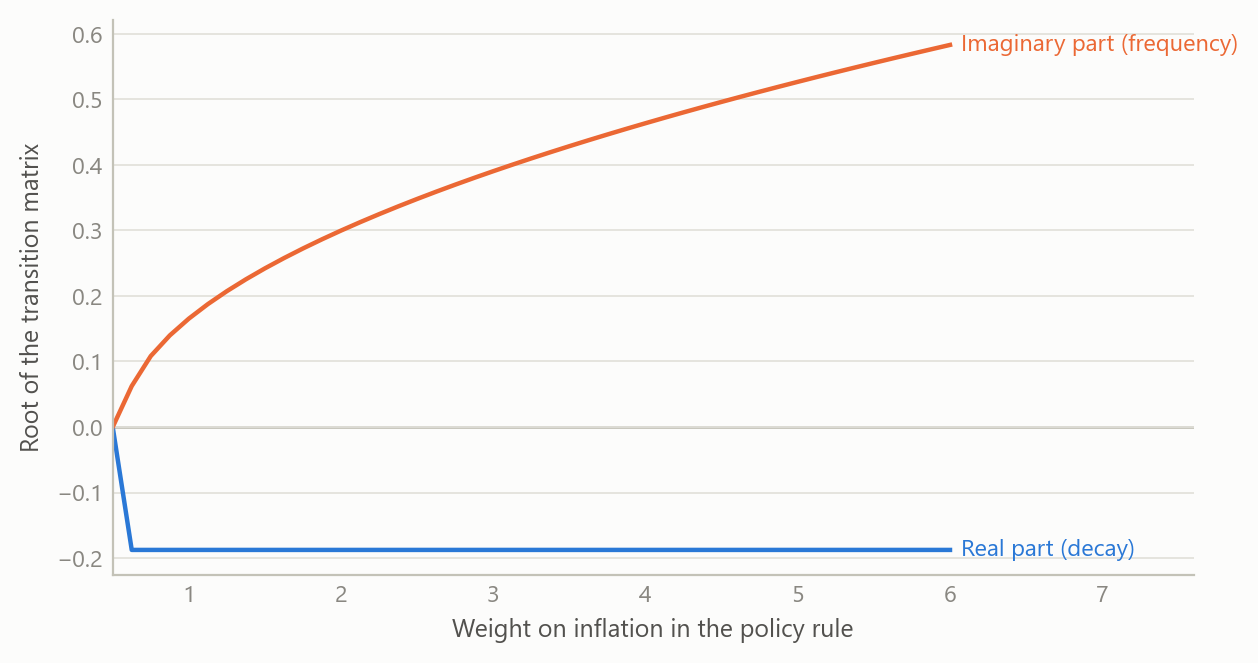
\includegraphics[keepaspectratio]{index_files/figure-latex/fig-roots-output-1.png}}

}

\caption{\label{fig-roots}Roots of the three-variable system as the
inflation weight in the policy rule rises (simulated data).}

\end{figure}%

\textbf{What a shock looks like.} A demand shock that decays over a few
quarters lifts output first, then pulls unemployment down, then raises
inflation; the rule responds and pushes everything back. The responses
are small and damped, and the rule brings all three back to steady
state.

\begin{figure}

\centering{

\pandocbounded{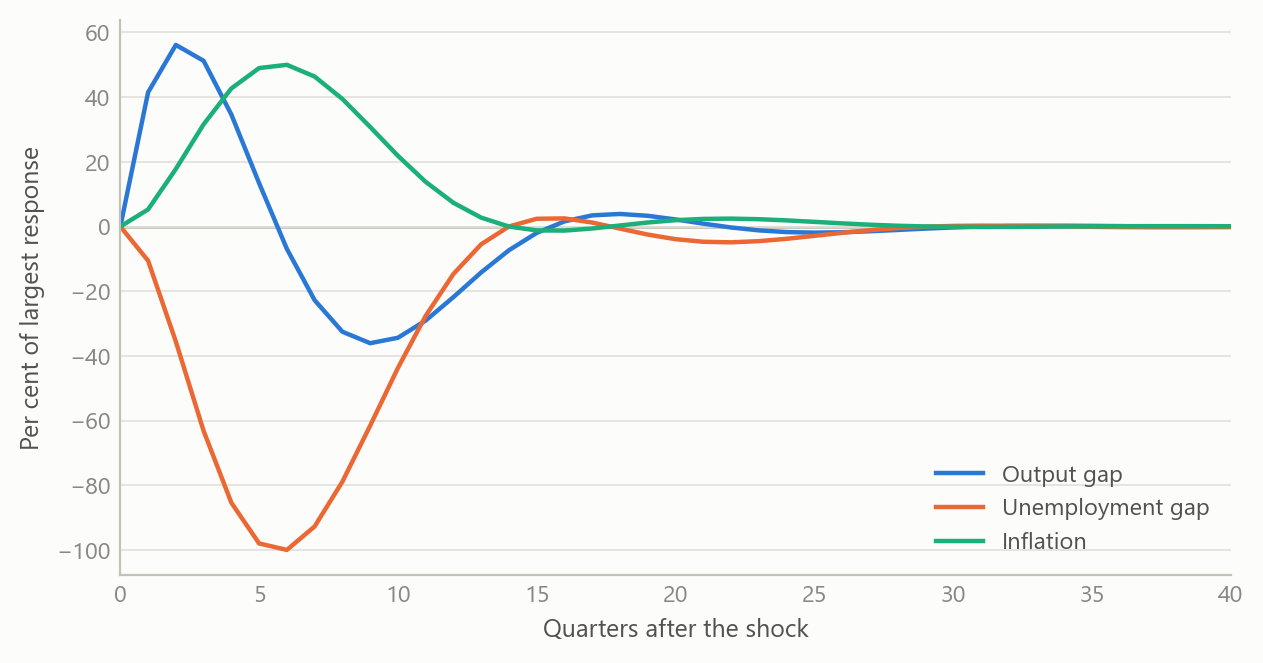
\includegraphics[keepaspectratio]{index_files/figure-latex/fig-irf-output-1.png}}

}

\caption{\label{fig-irf}Responses to a decaying demand shock: output
gap, unemployment gap and inflation, in per cent of the shock's peak
(simulated data).}

\end{figure}%

\textbf{From projection model to autoregression.} The derivation shows
the exact price of removing expectations: the resulting autoregression
is purely inertial. It is useful as a diagnostic benchmark, because any
gap between the full model's forecasts and the autoregression's is
attributable to expectations and policy behaviour. It is unsuitable for
forward-guidance questions, because without expectations a promised
future path of rates has no effect today. The notes also list the
minimum inputs needed to build the system: the series for each block,
their transformations to gaps, and the checks on quality and
stationarity.

\textbf{Debt dynamics.} The change in the debt ratio is the
interest-growth differential times the opening debt ratio, minus the
primary balance. Two implications follow from the algebra alone. First,
the primary balance needed to hold the ratio constant is the
differential times the debt ratio, so the same differential demands a
larger surplus the higher the debt. Second, when the differential is
positive the ratio compounds, and small shocks to the interest rate
matter more as debt rises. The figure shows the shape of this using
simulated paths.

\begin{figure}

\centering{

\pandocbounded{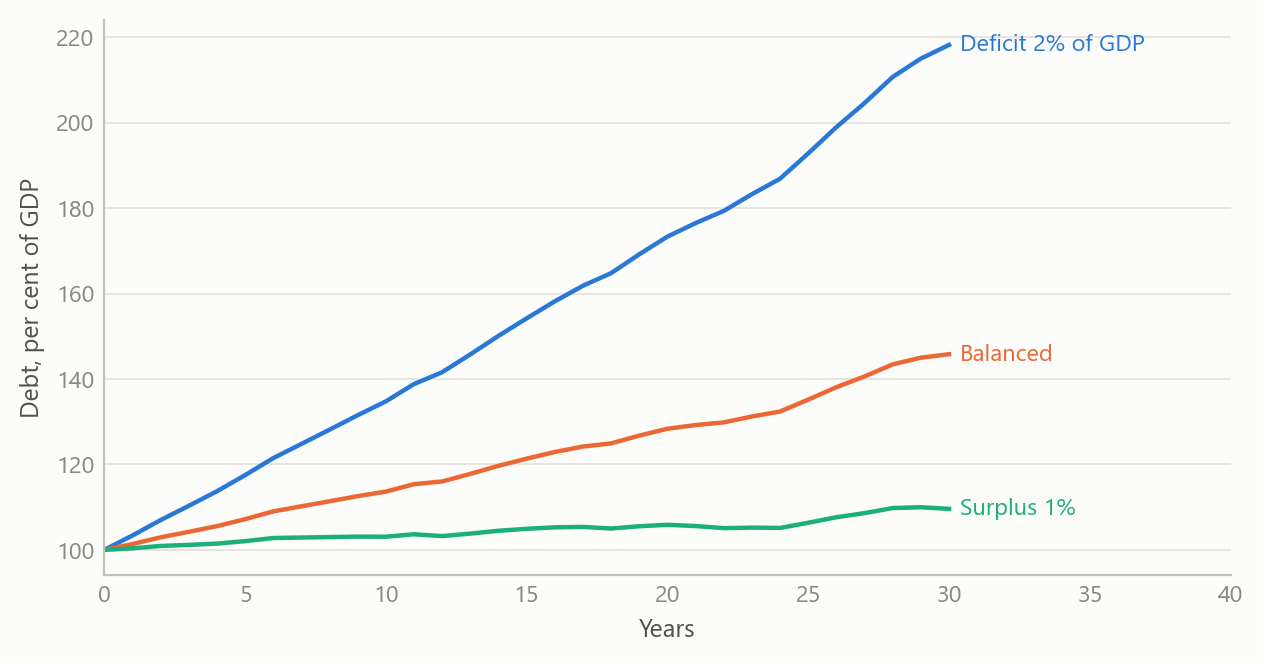
\includegraphics[keepaspectratio]{index_files/figure-latex/fig-debt-output-1.png}}

}

\caption{\label{fig-debt}Simulated debt-ratio paths for three
primary-balance settings, with a persistent, noisy interest-growth
differential (simulated data).}

\end{figure}%

\subsection{Insights}\label{insights}

\begin{itemize}
\tightlist
\item
  \textbf{Derivation exposes what a table of coefficients hides.} The
  finding that the decay rate does not depend on the inflation weight is
  invisible in a calibration table and obvious in the polynomial.
\item
  \textbf{Stocks and flows are a discipline, not a footnote.} Treating
  levels as integrals of flows is what makes the zero root appear, and
  what makes the discrete trace match the continuous system.
\item
  \textbf{Stability is a property of the whole loop.} For the
  three-equation core in its New Keynesian form, the standard
  requirement that the policy rate respond more than one-for-one to
  inflation is what stops expectations from becoming self-fulfilling;
  the notes show where in the loop that requirement bites.
\item
  \textbf{Removing expectations is a modelling decision with a known
  cost.} The implied autoregression is a clean benchmark precisely
  because it is blind to policy credibility.
\item
  \textbf{Pedagogy and audit are the same thing.} Writing each step so a
  newcomer can follow it is also the fastest way to find the step that
  does not follow.
\end{itemize}

\subsection{Scope and next steps}\label{scope-and-next-steps}

These are derivation and explanation notes, not estimation. The
coefficients in the worked examples are illustrative calibrations,
chosen to make the algebra concrete; they are not estimates from data
and should not be read as such. The three-equation system is
closed-economy and uses a single shock. The projection-model notes
derive the autoregressive form and set out the inputs it needs, but do
not report an estimated model.

The explanatory notes on the New Keynesian model and on debt dynamics
were built partly from secondary reading, and any empirical magnitudes
quoted there would need to be re-checked against primary data before
being relied on; they are not used here. The natural next steps are to
estimate the quarterly system on real data, to test the autoregressive
benchmark against out-of-sample forecasts, and to extend the debt
identity with a stochastic differential and a fiscal reaction function.

\subsection{About the evidence}\label{about-the-evidence}

The real content of this project is the derivations and the numerical
checks of them, written in 2025. The numbers quoted in the text are the
calibrated parameters and the roots computed from them; they come from
the notes' own numerical appendix. All figures in this page are
simulated, and the debt paths in particular are illustrative.

Figures and tables marked \emph{simulated} are generated from simulated
data built to share the structure of the analysis (its variables,
horizons and frequencies). They show how each method works and what its
output looks like. Results stated in the text, and figures that give a
source, are the project's own. Methods are described at the level of a
methods section. Code and data pipelines are not reproduced here.




\end{document}
